\chapter{Evolutionary optimization for the Kinoshita closure}
\label{Cap5}

In the previous chapter, a neural network was used to approximate the bridge function in 
the solution to the Ornstein-Zernike (OZ) equation. From the results obtained, it was 
implied that, without any more physical information, the neural network reduced its 
approximation to the well-known Hypernetted Chain closure relation. In this chapter, the 
modified Verlet bridge function is introduced, along with its variation, the Kinoshita 
closure. This bridge function contains more information in terms of the indirect 
correlation function, \(\gamma(r)\), which provides a more accurate solution when dealing 
with the hard-sphere fluid. Still, the Kinoshita closure is not thermodynamically 
consistent. Thus, in this chapter, the proposal of parametrizing the Kinoshita is 
introduced. These parameters are then fitted using Evolutionary Computation (EC) method for 
derivative-free optimization tasks. This is in the same spirit as with the 
Rogers-Young~\cite{rogersNewThermodynamicallyConsistent1984b} and the 
Zerah-Hansen~\cite{zerahSelfConsistentIntegral1986} closure relations. The goal of this 
proposal is to alleviate the problems that using a neural network has, in terms of 
incoporating more Physics into the modeling, instead of relying on the neural network to 
learn something by its own.

\section{The Kinoshita closure and its parametrization}
The proposal in this chapter deals with the modified Verlet closure and a variation of 
this, the Kinoshita modification. Both of these closure relations have been formulated to 
deal with the hard-sphere fluid, for low and large density values. The purpose of this 
section is to look at these closure relations more closely, as well as to define the 
parametrization to be used in later computations and results.

\subsection{The modified Verlet bridge function approximation}
Between 1980 and 1981, Loup Verlet published two papers were he introduced what is now 
called the \emph{modified Verlet} bridge 
function~\cite{verletIntegralEquationsClassical1980,verletIntegralEquationsClassical1981}. 
The idea behind his bridge function approximation was to derive a good approximation based 
on reproducing the exact first five virial coefficients of the hard sphere equation of 
state. The original proposition for the bridge function by Verlet was,
\begin{equation}
    B(r) = - \frac{A \, \gamma^{2}(r) \, / 2}{1 + B \, \gamma(r) \, / 2}
    \; .
    \label{eq:verlet-params}
\end{equation}
By fitting the exact values of the virial coefficients, Verlet reached the conclusion that 
the values for \(A, B\) that could reproduce the results for the hard-sphere fluid up to 
the fluid-solid transition where the values of,
\begin{equation}
    A = 1 \, , \quad B = \frac{4}{5}
    \; ,
    \label{eq:ab-verlet}
\end{equation}
which turns the original closure relation in \autoref{eq:verlet-params} into,
\begin{equation}
    B(r) = - \frac{0.5 \, \gamma^{2}(r)}{1 + 0.8 \, \gamma(r)}
    \; .
    \label{eq:mVerlet}
\end{equation}
This turned out to be an accurate bridge function approximation for the case of the 
hard-sphere fluid, even when hard sphere mixtures are 
considered~\cite{lopez-sanchezDemixingTransitionStructure2013a}.
Some of the advantages of this approximation is the fact that it is simple, efficient and 
there are no free parameters to be fixed, as is the case in the 
Rogers-Young~\cite{rogersNewThermodynamicallyConsistent1984b} and the 
Zerah-Hansen~\cite{zerahSelfConsistentIntegral1986} closure relations. The problem lies, as 
with other closure relations, with the fact that the bridge function in 
\autoref{eq:mVerlet} is not thermodynamically consistent. There are other closure relations 
which are already thermodynamically consistent, as is the case of the reference Hypernetted 
Chain approximation~\cite{ladoSolutionsReferencehypernettedchainEquation1983}. This 
approximation comes from first principles, and the thermodynamic consistency comes from the 
fact that the reference potential is chosen such that the free energy of the fluid is 
minimized. Still, the problem with this closure relation, although accurate, is that is 
might be hard to implement and use in several different scenarios.

\subsection{The Kinoshita variation}
For this reason, the idea of this chapter is to use the modified Verlet approximation, and instead of using the fixed parameters found from theoretical arguments, to let an evolutionary algorithm find the best ones that can also establish thermodynamic consistency. For this reason, the Kinoshita variation~\cite{kinoshitaInteractionSurfacesSolvophobicity2003} to the modified Verlet closure relation is introduced. This variation reads,
\begin{equation}
    B(r) = - \frac{0.5 \, \gamma^{2}(r)}{1 + 0.8 \, \left\lvert \gamma(r) \right\rvert}
    \; ,
    \label{eq:kinoshita-eq}
\end{equation}
and introduces the absolute value \(\left\lvert \cdot \right\rvert\) in the denominator, 
which increases the numerical stability of the closure relation for the case when there are 
very large and negative values of \(\gamma(r)\). However, in this case, the idea is to leave the original form of the closure relation, that is with two free paramaters,
\begin{equation}
    B(r) = \frac{\alpha \, \gamma^{2}(r)}{1 + \beta \, \left\lvert \gamma(r) \right\rvert}
    \; ,
    \label{eq:kinoshita-params}
\end{equation}
and instead look for the best values of both \(\alpha, \beta\) that yield an accurate 
result for the case of the isotropic hard sphere fluid in three dimensions.
To find these values, partial thermodynamic consistency will be enforced through the use of 
the pressure equations, which shall be discussed next.

\section{Thermodynamic consistency}
An important part of the results from this chapter is the notion of 
\emph{thermodynamic consistency}, the way it works and how it is implemented numerically. 
This is the goal of the present section.

When approximations to the bridge function are used, together with the OZ equation, most of 
the time the solution show a phenomenon where, if a thermodynamic observable is computed 
through two or more \emph{routes}, the results may vary drastically. This is not wanted 
behavior from the closure relations. Rather, it is expected that the closure relations 
could, in fact, provide accurate results regardless of the route they are computed with.
In section \autoref{sec:thermodynamics}, some of the ways to compute thermodynamic 
quantities using the radial distribution function, \(g(r)\), were presented. These will be 
presented here once more for the sake of clarity. Specialy, it is important to mention the 
two main routes that will be used later, the \emph{virial route} and the 
\emph{compressibility route}.

From \autoref{eq:pressure-equation}, the pressure equation for a $3$-dimensional fluid is,
\begin{equation}
    P = \frac{\rho}{\beta} - \frac{2 \pi \beta \rho}{3} \int_{0}^{\infty} u'(r) \, g(r) \, r^3 \, dr \, ,
    \label{eq:pressure-gr}
\end{equation}
this equation is also known as the \emph{virial equation} because it can be derived 
formally with the virial theorem (see \autoref{sec:thermodynamics}). Henceforth, 
this equation shall be known as the \emph{virial pressure equation}.

Another quantity of interest is the \emph{isothermal compressibility}, which was already 
introduced in \autoref{sec:thermodynamics}, and can be computed using the \(c(r)\) function 
as follows~\cite{hansenTheorySimpleLiquids2013},
\begin{equation}
    \frac{\beta}{\left( \chi_{T} \,  \rho \right)} = 1 - \rho \int d \vecr \, c(r)
    \; .
    \label{eq:compress-gr}
\end{equation}
For this reason, this equation shall be known throughout the rest of this thesis as the 
\emph{compressibility equation}. Using Thermodynamics, one can relate the pressure \(P\) of the system to the isothermal compressibility using the expression,
\begin{equation}
    \chi_{T} = - \, \frac{1}{V} { \left( \frac{\partial V}{\partial P} \right) }_{T} =
    \frac{1}{\rho} { \left( \frac{\partial \rho}{\partial P} \right) }_{T}
    \; ,
    \label{eq:chi-thermo}
\end{equation}
which is the same as in \autoref{eq:isothermal-chi}, again from 
\autoref{sec:thermodynamics}.

By enforcing that the pressure computed from \autoref{eq:pressure-gr} and the pressure 
computed from \autoref{eq:compress-gr} and then using \autoref{eq:chi-thermo}, are equal to 
some arbitrary precision, closure relations can be \emph{thermodynamically consistent}. 
This would mean that both routes will yield the same value. In reality, not many closure 
relations can do this, except for some special cases, which were already mentioned in the 
previous section. Thus, the standard way of alleviating the problem of thermodynamic 
inconsistency is to compute both these routes and adjust some parameter, or function, 
such that both routes provide the same result. It need not be just the pressure equations, 
also the energy equations can be used, as well as other thermodynamic quantities, such as 
the Helmholtz free energy or the chemical 
potential~\cite{tsedneeClosureOrnsteinZernikeEquation2019}.

\subsection{Numerical implementation}
In order to be able to compute the pressure from both routes, the \emph{virial} route and the \emph{compressibility} route, the following approach was followed.

For the case of the \emph{virial} route, \autoref{eq:pressure-gr} was computed as is, using 
the Romberg method for computing the integral~\cite{hammingNumericalMethodsScientists2012}. 
Due to the fact that the interaction potential is a continuous function (see 
\autoref{eq:cont-hs}), the exact derivative was computed and implemented. Then, to compute 
the isothermal compressibility from \autoref{eq:chi-thermo}, the derivative was 
approximated using a finite central difference scheme,
\begin{equation}
    \chi_{T}^{-1} = \rho { \left( \frac{\partial P}{\partial \rho} \right) }_{T}
    \approx \rho \lim_{\Delta \rho \to 0} \frac{P(\rho + \Delta \rho) - P(\rho - \Delta \rho)}{2 \, \Delta \rho}
    \; ,
    \label{eq:central-difference}
\end{equation}
where \(\chi_{T}^{-1}\) is the inverse isothermal compressibility. The notation 
\(P(\rho + \Delta \rho)\) means that, for a particular value of density given by 
\(\rho^{\prime}=\rho + \Delta \rho\), as well as for a fixed temperature \(T\), 
\autoref{eq:pressure-gr} was used to compute the 
pressure through the virial route. Here, \(\Delta \rho\) is a small value, fixed to be
\(\Delta \rho=\num{1e-10}\) in the results presented in this chapter. Other central 
differences were explored, such as the five stencil 
approximation~\cite{hammingNumericalMethodsScientists2012}, however, the results obtained 
were as accurate as those obtained with \autoref{eq:central-difference}, so there was no 
reason to justify the extra computational resources needed to do a five stencil difference 
scheme.

For the case of the \emph{compressibility} route, \autoref{eq:compress-gr} was computed as 
is, using once again the Romberg method for computing the integral.

\section{Black-box optimization problem implementation}
\begin{figure}
    \centering
    \vspace{-2cm}
    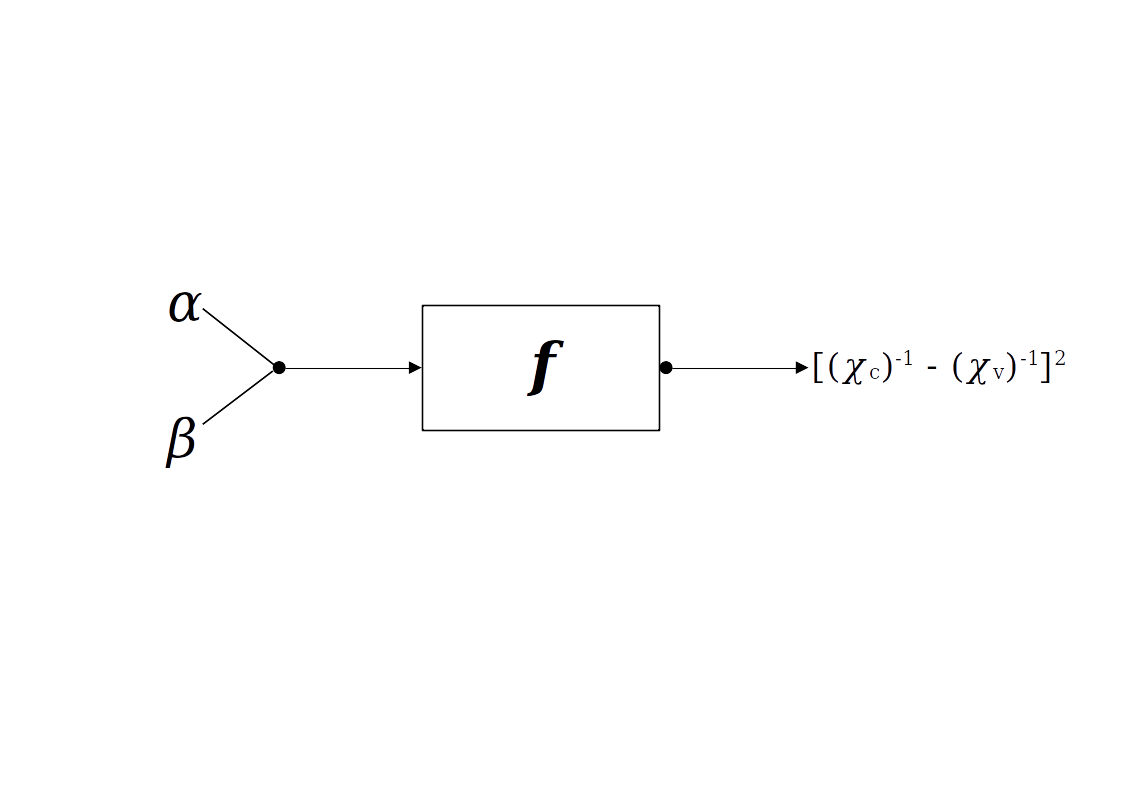
\includegraphics[scale=0.3]{figuras/capitulo-5/black-box-function.png}
    \vspace{-3cm}
    \caption{Schematics of the black-box function implementation. The function takes in two parameters, \(\alpha, \beta\), and yield the output given by the squared difference of the inverse isothermal compressibility through the virial and compressibility routes.}
    \label{fig:black-box-function}
\end{figure}

In order to solve the problem of finding the best set of values \(\alpha, \beta\) in 
\autoref{eq:kinoshita-params} that would provide thermodynamic consistency, a special type 
of setup must be implemented. It must be recalled that the main objective is for the virial 
and compressibility routes to provide the same value, thus, an \emph{optimization problem} 
can be setup. The problem can be formulated as an \emph{unconstrained optimization} problem,
\begin{equation}
    \underset{\alpha \, , \beta}{\text{minimize}} \: {\left[
        {\left(\chi_{T}^{c} \left(\alpha, \beta\right) \right)}^{-1} - {\left(\chi_{T}^{v} \left(\alpha, \beta\right) \right)}^{-1} \right]}^2
    \; ,
    \label{eq:optimiziation-chi}
\end{equation}
where \({\left(\chi_{T}^{c}\right)}^{-1}\) is the inverse isothermal compressibility 
computed through the \emph{compressibility} route; \({\left(\chi_{T}^{v}\right)}^{-1}\) is 
the inverse isothermal compressibility computed through the \emph{virial} route; and the 
notation \({\left(\chi_{T}^{c, v} \left(\alpha, \beta\right) \right)}^{-1}\) represents the 
dependency of the parameters \(\alpha, \beta\) that would yield such value of the 
compressibility. In other words, for a fixed set of paramaters \(\alpha, \beta\), the 
inverse isothermal compressibility is computed via both routes, and its difference squared 
is computed. The goal of the optimization problem is to \emph{minimize} this difference. If 
a good set of parameters is found, the the difference will be, ideally, zero or close to 
zero, which in turn would mean that both routes are providing the same results, up to an 
arbitrary numerical tolerance.

In order to perform the optimization procedure, all the necessary computation must be bundled together into a single \emph{black-box function}. This function, which is modeled in \autoref{fig:black-box-function}, will take as input two values and will output the difference between the inverse isothermal compressibility values computed using both routes. Thus, the function will perform the following steps:
\begin{enumerate}
    \item Take as input two fixed values, \(\alpha^{\prime}, \beta^{\prime}\), and use them to define the Kinoshita closure in \autoref{eq:kinoshita-params}.
    \item Solve the OZ equation (see \autoref{AppendixB}) with the closure relation provided in the previous step. This will output two important quantities, the radial distribution function, \(g(r)\), and the direct correlation function, \(c(r)\).
    \item Using \autoref{eq:pressure-gr} and the details presented in the previous section, \({\left(\chi_{T}^{v}\right)}^{-1}\) is computed.
    \item Then, using \autoref{eq:compress-gr} and the details presented in the previous section, \({\left(\chi_{T}^{c}\right)}^{-1}\) is computed.
    \item After both routes have been computed, its squared difference is computed, i.e., \({\left[ {\left(\chi_{T}^{c} \left(\alpha, \beta\right) \right)}^{-1} - {\left(\chi_{T}^{v} \left(\alpha, \beta\right) \right)}^{-1} \right]}^2 \).
\end{enumerate}
Thus, the previous steps comprise the \emph{black-box function} shown in 
\autoref{fig:black-box-function}, which will later be minimized.

\subsection{Optimization procedure}
To solve the optimization problem in \autoref{eq:optimiziation-chi}, Evolutionary 
Comptuation methods were employed. However, there are two parts to the solution of this 
problem. First off, the function is treated as a \emph{black-box function}, which means 
that no derivatives can be computed, and that it is assumed that each function evaluation 
is costly. Although the numerical methods are quite optimized, it is safe to assume that 
each function evaluation is costly, and use this argument to select a good optimization 
method that can effectively reduce the number of function evaluations.

For this reason, Evolution Strategy methods were employed, in particular, Natural Evolution 
Strategies (NES) (see \autoref{Cap3}). These methods are robust, albeit slow to reach a 
minimum. 
Furthermore, these methods are \emph{global optimization methods}, meaning that these 
method will only look for global values throughout the function lanspace, and if any minima 
is found, it will not look deeper into that particular set of parameters. For this reason,
\emph{local optimization methods} are used, to perform a more exhaustive search into the 
previously found global minima. Thus, the optimization procedure looks like the following,
\begin{enumerate}
    \item Select an initial search space of \(\left[-75, 75\right]\) for each parameter, and choose an initial set of parameters randomly from within the search space.
    \item Using the DXNES global optimization method~\cite{nomuraDistanceweightedExponentialNatural2021}, perform a search for all the global minima in the interval \(\rm{x} \in \left[a, b\right]\).
    \item Keep the minima that satisfy the condition \(\rm{x} \leq 0.5\).
    \item Using a local optimization method, the BOBYQA method~\cite{powellUOBYQAUnconstrainedOptimization2002}, take as input the parameters found by the previous two steps, \(\rm{x}^{\prime}\). Use these within a shorter interval of \(\pm 5\) for each parameter, and look for a new set of parameters.
    \item Stop the optimization procedure when the new set of parameters satisfy the condition \(\rm{x}^{*} \leq \num{1e-7}\).
\end{enumerate}

To see this more clearly, an example is worked out now. First, a density value is fixed, 
\(\phi = 0.4\), and all the necessary parameters to solve the OZ equation are fixed as 
well. Then, the search is space is fixed to be \(\rm{x} = \left(\alpha, \beta\right) \in \left[-75, 75\right]\). 
An initial set of parameters is chosen randomly from within this search space, for 
instance, \(\rm{x} = \left(-10, 42\right)\). These pair of values are then fixed to be the 
value of \(\alpha, \beta\) in \autoref{eq:kinoshita-params}. With these new values, the 
closure relation is fixed and the OZ equation is solved. If the OZ equation can be solved 
using these values, then the result of the OZ equation is the pair of functions 
\(g(r), c(r)\). Using these values, and the details from the previous section, the squared 
difference 
\[
    \Delta \chi^{-1}_{T} = {\left[ {\left(\chi_{T}^{c} \left(\alpha, \beta\right) \right)}^{-1} - {\left(\chi_{T}^{v} \left(\alpha, \beta\right) \right)}^{-1} \right]}^2 
\; ,
\] 
is computed, and the global optimization method registers this value. If the value 
\(\Delta \chi^{-1}_{T}\) satisfies the condition \(\Delta \chi^{-1}_{T} \leq 0.5\), then 
the set of values \(\rm{x} = \left(-10, 42\right)\) is used for the local optimization 
method. However, in this case, the search space is bounded about these values by a factor 
of \(5\). In this example, that would mean that the new search space for the local 
optimization method would be \(\alpha \in [-15, -5]\) for the first parameter, and 
\(\beta \in [37, 47]\) for the second parameter. Then, the local optimization method would 
start looking for the minimum in this search space, and when a set of values satisfy the 
condition \(\rm{x}^{*} \leq \num{1e-7}\), then the optimization procedure has converged, 
and the set of values are regarded as the best values that provide thermodynamic 
consistency.

\section{Results}

\section{Discussion}

\section{Concluding remarks}